\chapter{Implementation}
\label{ch:implementation}

\section{Project Management}
The table below is the initial project timetable set out in the project specification document. It was used as a rough guide to keep the project on track by helping know what tasks needed to be done and for how long. 

\begin{center}
	\begin{tabular}{ | c | l | }
		\hline
		\textbf{Dates} & \textbf{Event} \\ \hline
		T1 W1-2 & Project specification \\ \hline
		T1 W1-2 & Research into development tools \\ \hline
		T1 W3-9 & Development of website foundation \\ \hline
		T1 W4 & Design basic UI \\ \hline
		T1 W5-7 & User authentication \\ \hline
		T1 W8-9 & Integration with PlaidAPI \\ \hline
		T2 W1 & Testing of website foundation \\ \hline
		T2 W2-10 & Repeated strategy development \\ \hline
		Easter & Finishing touches \\ \hline
		Throughout & Document research \\ \hline
		T3 W1 & Dissertation due \\ \hline
	\end{tabular}
\end{center}

Following the submission of the progress report, it was made clearer that the project had four key phases. The first phase was research into the development methodologies and design. The second phase was the development of two proof-of-concepts and merging them into a single application, following the waterfall methodology. The third phase was repeated strategy implementation and testing, following an agile methodology. The final phase adding the budget prediction as a separate major feature. These divisions were a simple progression from the original timetable and were more natural with the whole project schedule by that point.

\subsection{Research and Design}
Most of the findings in this section have been outlined in the previous chapters (\ref{ch:background}, \ref{ch:design}), but it is still worth talking about how the research was conducted and the structure of this process. This phase was performed prior to the progress report and change in timetable, so aligned with the original project specification.

Initially, only the aim of the project and the plan to use open banking was set in stone. In early term 1, research into how open banking is performed and how a developer could utilise the service was the main priority, this is when the discovery of Plaid was made, and the decision to use it happened. With familiarisation and proficiency in Next.js, it was a clear choice to use as the framework, and lots of the other design decision were made from understanding how to use Plaid.

Plaid is a relatively new technology, but it is still like any framework so to understand how to use it, a common research methodology was used. Vinicius' article \cite{FrameworkLearning} talks about the best method for learning a new language or framework and has almost ten-thousand claps (the measure of popularity of Medium), so many people agree. The article is a good summary of the process and the main points which were followed when learning Plaid were: start with the basics, read lots of documentation, find examples on GitHub and Stack Overflow, and finally build something. In addition to this, due to Plaid having an YouTube channel \cite{PlaidYouTube}, watching videos was also added and provided an effective way to learn. 

Plaid had a getting started video, which helped explain the basics of the service as well as the terminology used in the documentation. Following this, lots of the documentation was read to not only help when coding, but also to understand what features were available and how they could be used to build financial capability. Due to the recency of the revised way Plaid works, there are few example of how to use it on GitHub, and almost no questions on Stack Overflow; however, as part of the Plaid getting started video, they provide a code repository with a basic implementation of Plaid which helped to understand the service. Learning how to use Plaid helped inform lots of other design decisions, for example the Plaid authentication flow dictated the need for separate frontend and backend services to be developed, as well as the need for a database to store the user's credentials.

The other major development technologies that were researched here included Next.js features that had not been used before, such as server side rendering, as well as the combination with TailWindCSS and the use of PocketBase. The research into these technologies was done in a similar way to Plaid as it have proven to be effective. The main difference is that there is much more documentation and resources available for these so was slightly easier to learn. As well as technologies, concepts had to be learnt such as how authentication should be performed to ensure that user information is kept secure and how to follow modern web development best practices to build a successful web application.

The final point in Vinicius' article was to build something. This is the major reason which influenced the next phase of the project to be building two proof of concepts to test and improve the knowledge of the technologies and concepts learnt, but also provided a good basis for the actual application itself.

\subsection{Proof of Concepts}
To put the research from the previous phase into practise and work with the new technologies, this phase was to build two separate proof of concepts, one to have basic user authentication and the other to be able to interact with the Plaid API. Once both the prototypes were built, they would be merged into one application and form the basis for the rest of the project.

This phase of implementation is where there was first deviation from the original plan in the specification. In this instance, the development followed the waterfall methodology. This was because it lent itself nicely in the way this phase was structured. Having the knowledge of what the technologies can do, and having a clear goal for each proof of concept, a clear step-by-step plan could be constructed. In addition, there was only a single developer so the waterfall methodology was a good way to ensure that the project was on track and that the developer was not overwhelmed with too many tasks at once. Waterfall is known for being effective in projects that have concrete objectives set out from the beginning. Both applications were worked on the same time, performing each stage of the waterfall process for both applications. This was done to ensure that the applications could also interact with each other when the time came to merge them. For example the second stage of waterfall is design, so both the designs for the applications were set out at the same time, and both before the implementation (the next stage).

This sequential process is easy to manage but does not perform well for unexpected changes. This meant that the original requirements had to be detailed enough to encompass any possible queries, as well as have some contingency plans in place. For example, from some initial research, Plaid's endpoints could take in an array of accounts to return the transactions for all of them, however online elsewhere, someone had mentioned that this often just failed. To account for this, the plan was to use the Plaid endpoint, however if it didn't work, there also was a plan and design in place to manually query the endpoint for each account, which would functionally be the same.

\subsubsection{User Authentication}
User authentication was needed to only allow logged in user's to access their dashboard, and only each logged in user can access the transactions for the access\_tokens which they created. The design for this application was to have three pages. The first page would be the signup page, where they can create an account. The second page would be the login page, where they can login to their already created account. The final page would be the dashboard which displayed the user's email if they were logged in, and would redirect to the login page if they were not. The signup page and login page would have links to each other so that the user could navigate between them.

The implementation for the user authentication was simple yet secure. Both the signup page and login page have two inputs for the email and password, along with a submit button for the form. When a user creates an account, firstly the client checks that the email is a valid and unique email, and that a password has been entered. If so, the database is then populated with the new account and the user is sent to their dashboard. If the email is not valid or unique, the user is notified of this via an error message. The creation of user's account, as well as when performing the logging in is done using the PocketBase npm package, which automatically hashes and salts the passwords for security.

The login page works in a similar way, but instead of creating a new account, just checks that the entered email and password match an account in the database. If so, the user is sent to their dashboard, if not, they are notified of the error via a message on the page. On the dashboard page, the user is checked to be logged in via the PocketBase authStore, which uses JSON Web Tokens (JWT) under the hood. This means they can hold the user's ID and allows the database to limit access to the user's data by only allowing requests that come from that user. The ID is stored encrypted in the JWT, which itself is stored encrypted in a cookie. In addition, the JWT is only valid for a short period of time, to avoid cases where the cookie is stolen and the user's account can be accessed by someone else. Security is a major concern for this project as it handles sensitive financial data.

\begin{figure}[H]
	\centering
	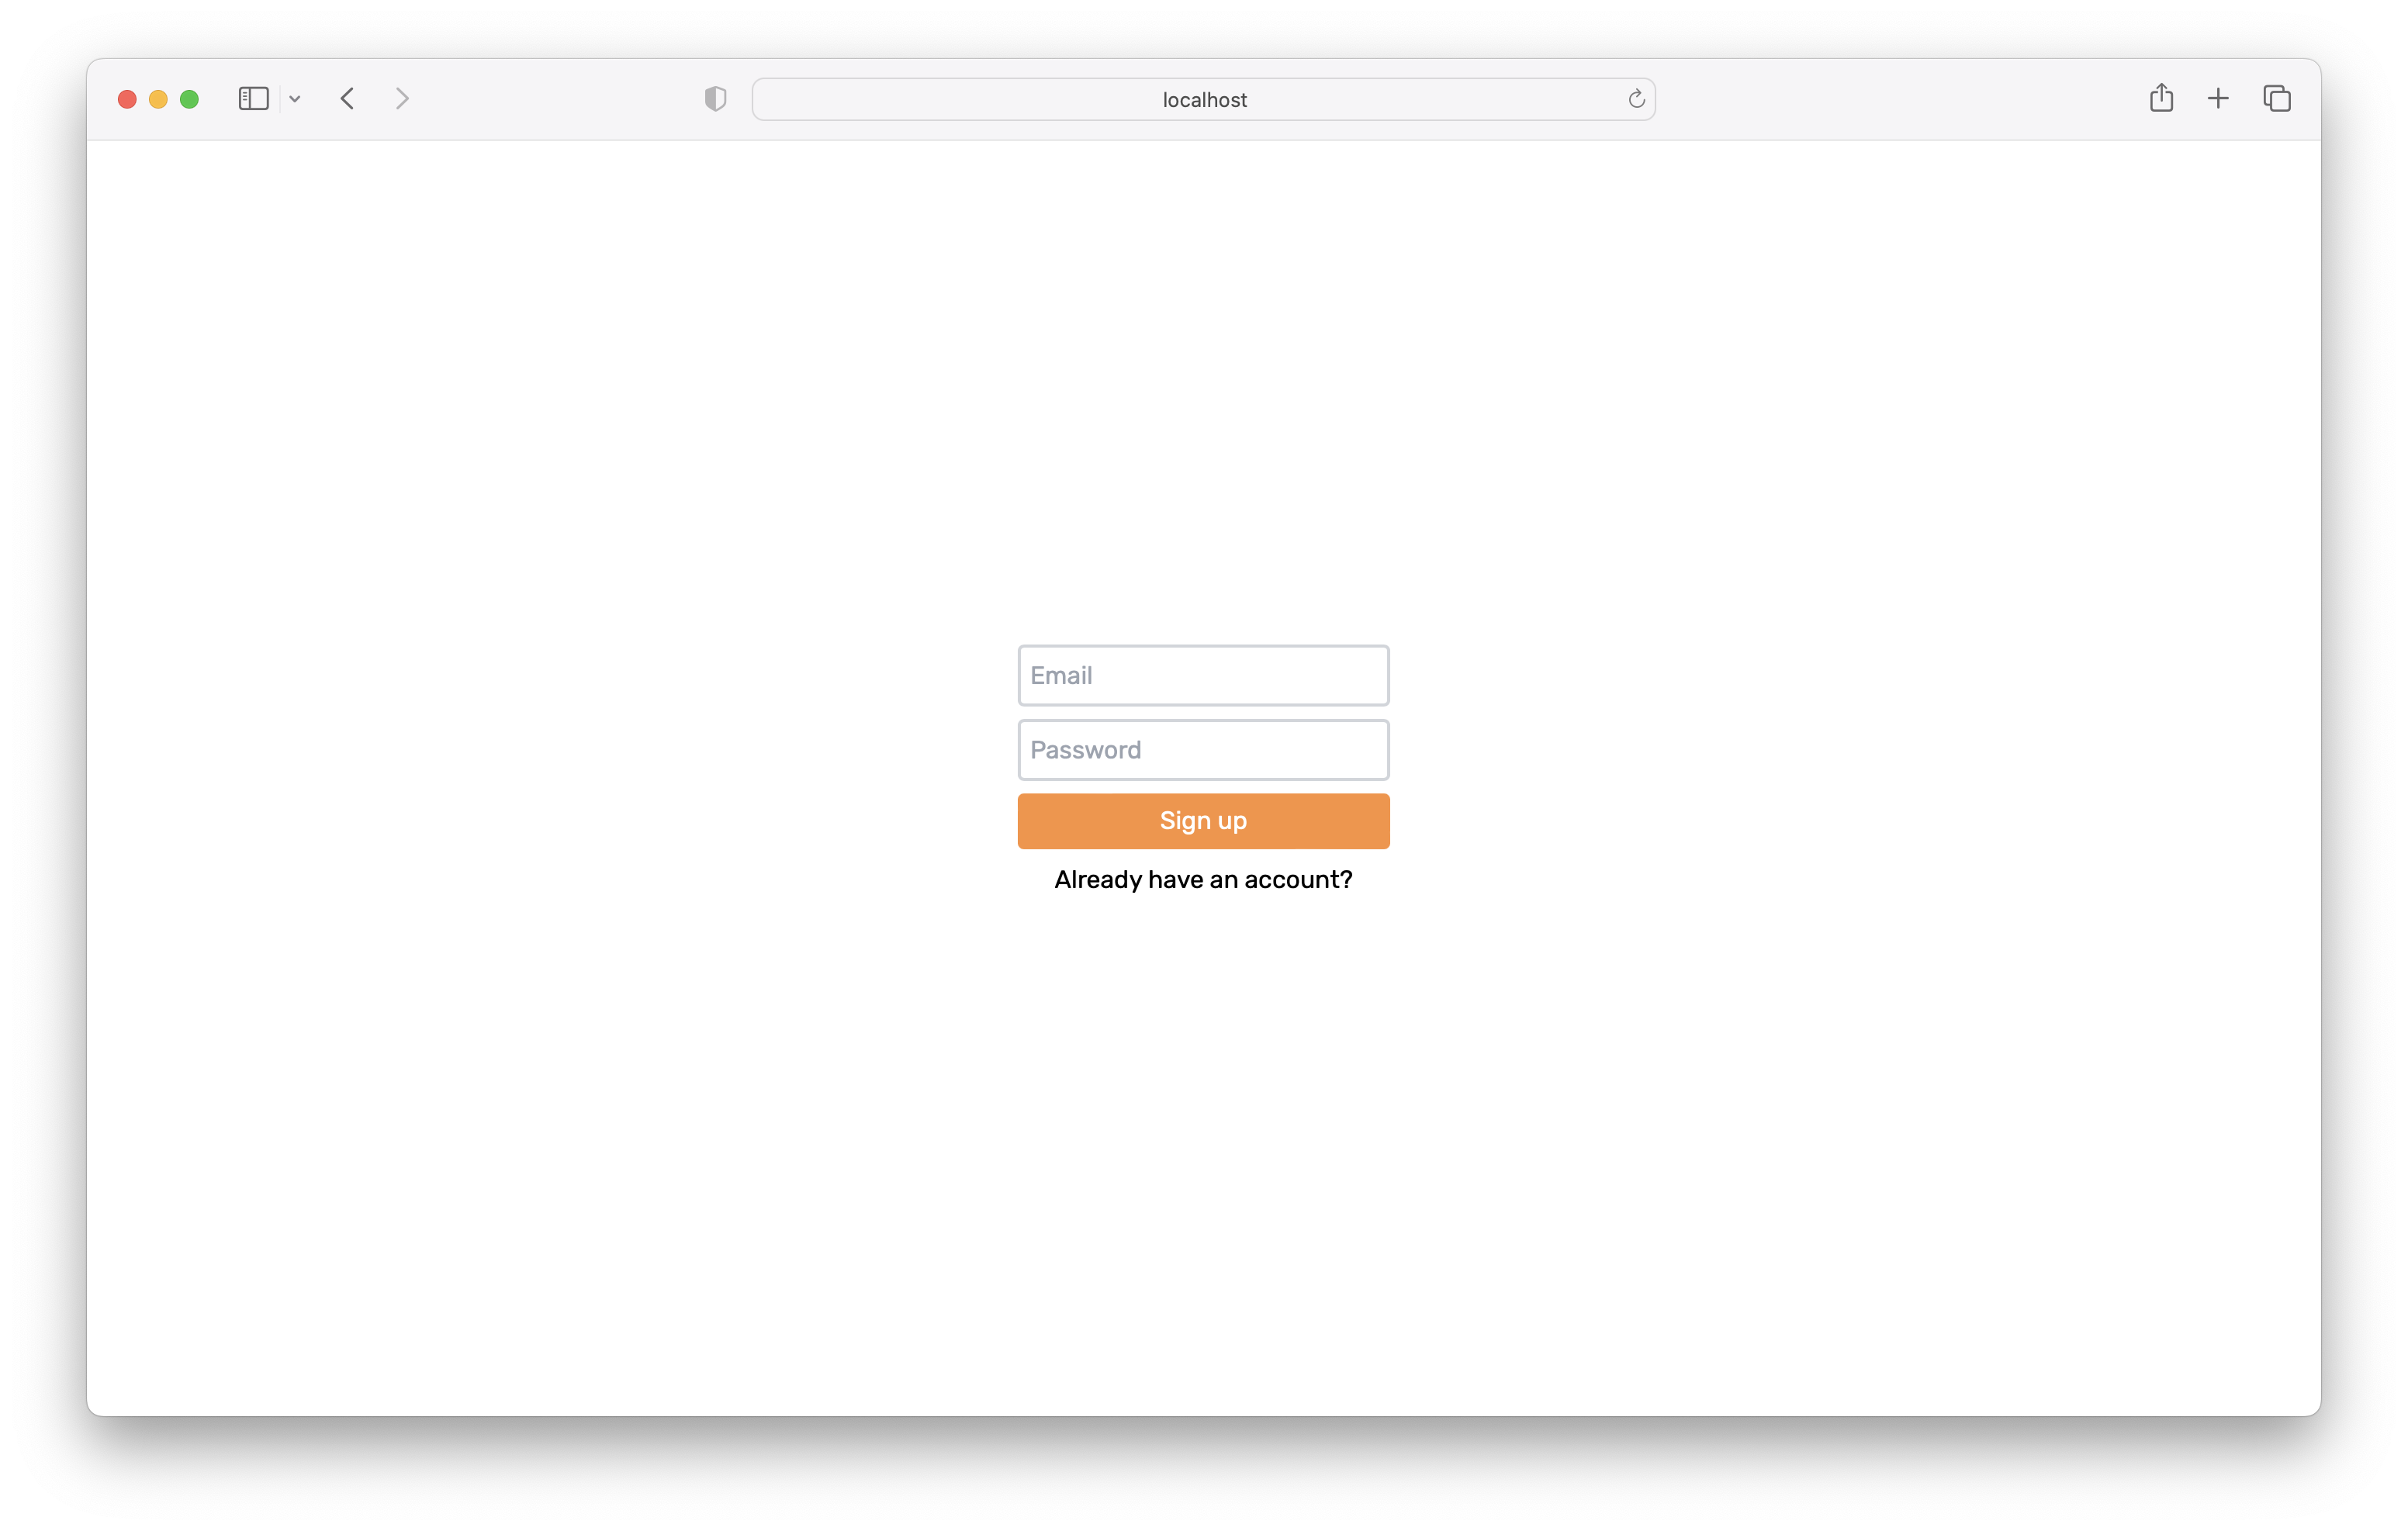
\includegraphics[width=\textwidth]{images/Signup_page.png}
	\caption{The minimal signup page for the user authentication}
	\label{fig:Signup_page}
\end{figure}

\begin{figure}[H]
	\centering
	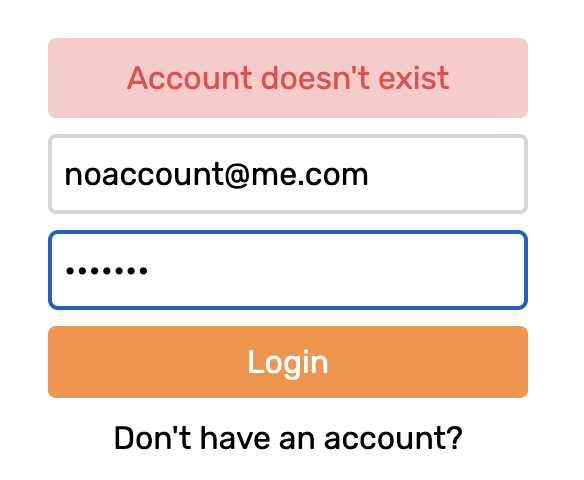
\includegraphics[width=0.5\textwidth]{images/Noaccount.png}
	\caption{The login component, with an example error message}
	\label{fig:Login_component}
\end{figure}

\begin{figure}[H]
	\centering
	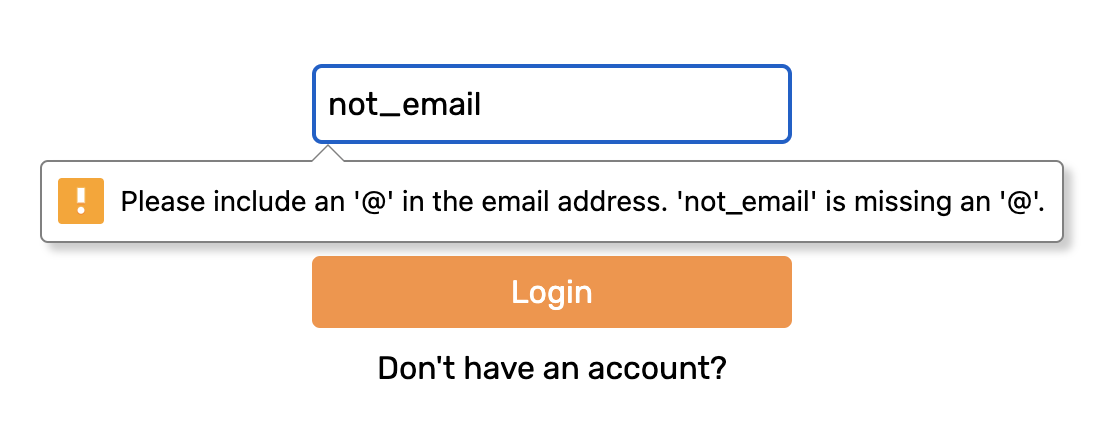
\includegraphics[width=0.9\textwidth]{images/email_validation.png}
	\caption{The client-side validation for the email input}
	\label{fig:Email_validation}
\end{figure}

\subsubsection{Plaid API}
The second proof of concept was to be able to interact with the Plaid API. The design was to allow a user to follow the authentication flow of Plaid and link a bank account, this results in getting an access\_token. Then, using the token, access their recent transactions. To begin the process, a user would click on a button to request the link token and have the link widget popup. The rest of the authentication flow would be as described in the background section (\ref{ch:background}), and after linking the access\_token would just be stored client side for now.

This system required minimal design and little styling as the authentication flow is dictated by Plaid themselves, and the aim of this proof of concept was just to have functionally, so no need for fancy looking components. Again as using the waterfall methodology, the implementation was also simple. From the previous research, the whole process was already known and so from the complete plan created in the stage before, there was little deviation.

\subsubsection{Merging}
At this stage, there were two independent proof of concepts that served different purposes, however the aim for the project was to have one working application that does what both of them do, and more. Both the proof of concepts had been written using git, but where on separate branches. The basic user authentication was deemed more fragile, so it was decided to merge the Plaid interaction into that application. The idea was to have the user first perform the basic authentication, then on the dashboard they could link their bank accounts, and then for each access\_token generated, this was to be stored in the database. Furthermore, on the dashboard, if that user already had an access\_token available, they could request their transactions and they would just be displayed in the console.

With the waterfall methodology, and having the knowledge of how to implement these systems already independently, each stage could, and was, meticulously planned so the merge went smoothly and the bare-bones application was ready for the strategies to be added. The only new feature, not in either was the ability to store the access\_token in the database, and retrieve it when doing the transaction query; however, this was not that difficult from performing the user authentication such as getting the user's email/password, and it is a common task so there were lots of resources online to help.

During the implementation, something that was not considered was when a user has multiple access token and what to do. This oversight was easily mitigated, as the rest of the functionality was implemented in accordance with the original plan. Then as an extra a slight modification was made afterwards that when requesting the transactions, instead of getting the first access\_token, it instead returns all the access\_tokens, and then for each a query is made to Plaid. This is different to a user having multiple bank accounts linked, as each access\_token can contain multiple bank accounts, but the ability to toggle the individual bank accounts was not worried about at this stage.

\subsection{Repeated Strategy Implementation}
At this stage, the application was extremely basic and only had the ability to link bank accounts and retrieve transactions. The actual strategies to help improve financial capability were yet to be added or even designed. This was a separate major phase in the project and instead of using the waterfall methodology, an agile methodology was more appropriate and so used. It wasn't any particular sub-methodology like scrum or lean, but instead just had very agile practises as was worked on in sprints. Each sprint was for a different strategy and so they could be independently added, but would come together to form the final application. This separation was also shown during development as each strategy was developed on a separate branch, and then merged after passing the tests and being mostly complete.


\subsubsection{Agile Development}
In general, the waterfall methodology should be prioritised for a project of this scale and especially where there is only one developer. For the repeated strategy development, due to the nature of the requirements being difficult to define prior to each strategy, agile was more appropriate. Within each strategy, and therefore sprint, research into the how best to include the strategy to maximise financial capability. This meant that the actual plan for each strategy was not known until the research was complete, so unable to set clear objectives in waterfall. Similarly, agile allowed for each sprint to consist of this research, but then followed by the design and implementation. If any issues arose during the implementation, they could be easily managed by altering the design, if appropriate, due to the flexible nature of agile.

Initially it was decided that each sprint would be three weeks long, one week each for research, development, and testing. However, it was found that this gave too much time for each section and especially for research so was modified accordingly. Agile's ability to change on the fly was a major benefit, in particular for this example. The spring was reduced down to roughly ten days, where there was so set time for each section, but instead the time was split among the three. This was useful after completing the transaction strategy, and moving on to the categories strategy. Much less time needed to be spent on the research as there was some crossover, meaning more time could be spent on the implementation and testing.

\subsubsection{Credential Management}
Following the merged proof of concepts, the application was sent to Plaid to request development access (instead of sandbox). Thanks to the previous research, the authentication flow was strictly and securely followed such that the application was approved. As outlined in the background section (\ref{ch:background}), development access meant that real live financial information could be accessed and used. This was a major milestone, but also came with further things to manage. With development access, the application could have one-hundred access\_tokens in total. The credentials were therefore treated as a resource and were used infrequently to ensure that enough were available for the final testing stages and the demonstration in the presentation. To account for this, all unit tests were only ever run in sandbox mode and only once these were passed did integration testing begin. Integration testing was firstly done in sandbox mode, but then once happy, the same tests were performed in development mode. More often than not, no issues arose only in development mode, but it was still important to test in both modes to ensure that the application is reliable. 


\subsubsection{GitHub Flow}
As mentioned earlier, each strategy had its own branch and only merged once it was complete. This was in attempt to follow the GitHub Flow branching model \cite{GitHubFlow}. It involves having the main branch always deployable; all changes are made through separate feature branches via pull requests and merging; and rebases are used to avoid conflicts. The advantages include that multiple versions do not need to be managed, as well as that frequent changes can be pushed e.g. after every sprint, and the codebase is much cleaner to work with.

The original plan was to use the GitFlow workflow \cite{GitFlow} where there are develop and feature branches, however this workflow is aimed at more collaborative projects, as well as ones that need to have stable releases at set time periods. Furthermore, GitHub Flow offered the same advantages for a single developer, and was much less complex.

\subsubsection{MVP and Testing}
By the end of the repeated strategy implementation, a minimal viable product (MVP) was created that had the functionality to improve financial capability, but still had room for further features like budget prediction. Each individual component was thoroughly tested, as well as the integrations and pages as a whole. The individual component testing was often done in code and included the frontend as well as the backend, whilst the integration testing was mainly done manually. There was some integration tests completed in code, and all the automatic tests had to be passed before any branch was merged.

\subsection{Budget Prediction}
Following the repeated strategy implementation, there was a basic budgeting strategy, but it only displayed the expenditure so far in the current month and allowed the user to set a budget. The original aim was to increase financial capability, and a worthwhile feature that would do this would be to predict the expenditure and allow the user to adjust earlier, ultimately to make better decisions.

This was added as a separate major feature, unlike the previous strategies, because it was much bigger. A lot more research and planning was required for this as it would involve creating machine learning models, as well as, a separate server to host the model. By this time, only minor tweaks were being made to the MVP as hot-fixes, so the GitHub Flow workflow was followed again, by performing this in a separate feature branch.

The process for this feature was somewhat treated like another agile sprint, however it was not formalised like this, as going into the prediction, there was little certainty as to how effective it would be, or even what the requirements were outside of predicting future expenses.

Also as part of managing this section, the machine learning models would need real financial data for training to be the most accurate. This has some privacy concerns as the model would learn from the this data the information would be shown in the predictions. Furthermore, there was a limitation on the amount of financial data that could be accessed, so in the end it was decided to mix the data. The model was trained using only the developer's financial data as well as some of the data from Plaid's sandbox mode. This was in an attempt to still create a useful model, but to not leak any information and it not overfit on a single individual. In addition, some data manipulation techniques, outlined in the implementation, were used to simulate more data and make the model more robust.

\section{Strategies}
This section aims to outline the strategies that were implemented in the application. Only the final option that was decided in the design section will be explained. They were each implemented as independent sprints, however they all had the same goal of improving financial capability by providing the user with information and tools to make better financial decisions.

\subsection{Active Bank Accounts}
As part of the navigation bar show in figure \ref{fig:DashboardNavigationBar}, the rightmost button with the label 'accounts' is a dropdown. Clicking it displays a menu containing all the linked bank accounts, an add accounts button, and a logout button. Each linked bank account is a bar containing toggle button, the name and type of the account, and a logo representing which bank chain it is from. The add accounts button is where the user can link more bank accounts by beginning the Plaid authentication flow. The logout button is simply where the user can logout and the application will clear the cookie.

This was implemented as part of the transactions sprint as was not included in the initial proof of concepts, however is necessary for all the other strategies. All the bank accounts are active by default, however the user can toggle them off to not include them in the analytics. Each bank account has an associated id, and so a list of active bank account ids is stored as state in the navigation bar. This array is passed to each of the strategy components as a prop to filter the data and only include the active accounts.

\begin{figure}[H]
	\centering
	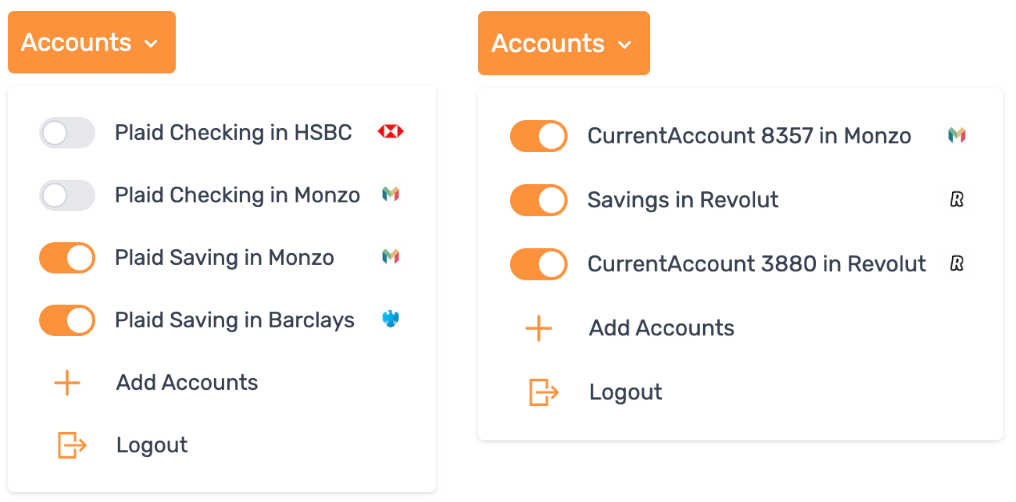
\includegraphics[width=\textwidth]{images/Accounts_dropdown.png}
	\caption{Account dropdown for (left) sandbox mode and (right) development mode}
	\label{fig:AccountsDropdown}
\end{figure}

In the above figure \ref{fig:AccountsDropdown}, the left image is from the sandbox mode and the right image is from the development mode. In sandbox mode, only the savings accounts have been toggled on, for example if a user wanted to only view the analytics for those accounts. In development all the bank accounts, which in this case is a Monzo and two Revolut accounts, are enabled. When switching between a toggled account, the icon has a slight animation.

\subsection{Transactions}
This was the first strategy implemented, so there was a lot of experimentation and learning how best to get the data from Plaid and propagate it to the frontend, then display nicely. Each strategy was implemented as a separate component and the data required, such as the user object and active accounts, were passed down as props in the React model. This meant that the dashboard would simply just render the component of the strategy currently being viewed.

The transactions strategy is implemented as a table where each row is a separate transaction to a merchant. The transactions are grouped by date and in reverse chronological order. When querying Plaid, it returns the transactions in order of the accounts, so some extra data preparation was needed.

A single Next.js API route was needed to be built. It would take only the user ID as a parameter, and query the database for all the access tokens associated with that user. It is only able to see the access tokens that it created, so in this case would just get all the access tokens. With these, it makes a request to Plaid to get the transactions for each access token. The transactions are then grouped and sorted in the API route, such that the frontend needs to do minimal work. The transactions are then returned to the frontend as a JSON object to be displayed.

Plaid has multiple endpoint's that access transactional data. To begin with, "/transactions/sync" was used which gets the transactions. The first call returns all the historical transactions (up to a limit) along with a cursor, subsequent calls update the cursor and only return transactions after the cursor. This reduces the amount of data flow and means the transactions can be stored locally for faster loading. On strategy load however, the UI needed to send a request to Plaid, and a request to the database

This ended up being changed to instead use "/transactions/get" which returns the transactions between an input start date and end date as the transactions didn't need to be stored. Plaid encourages to use the sync endpoint as it acts as a subscriber model and also paginates the data, however the get endpoint enabled code reuse for later strategies, withdrew the dependency on the database, and also reduced the number of requests when loading the strategy.

\begin{figure}[H]
	\centering
	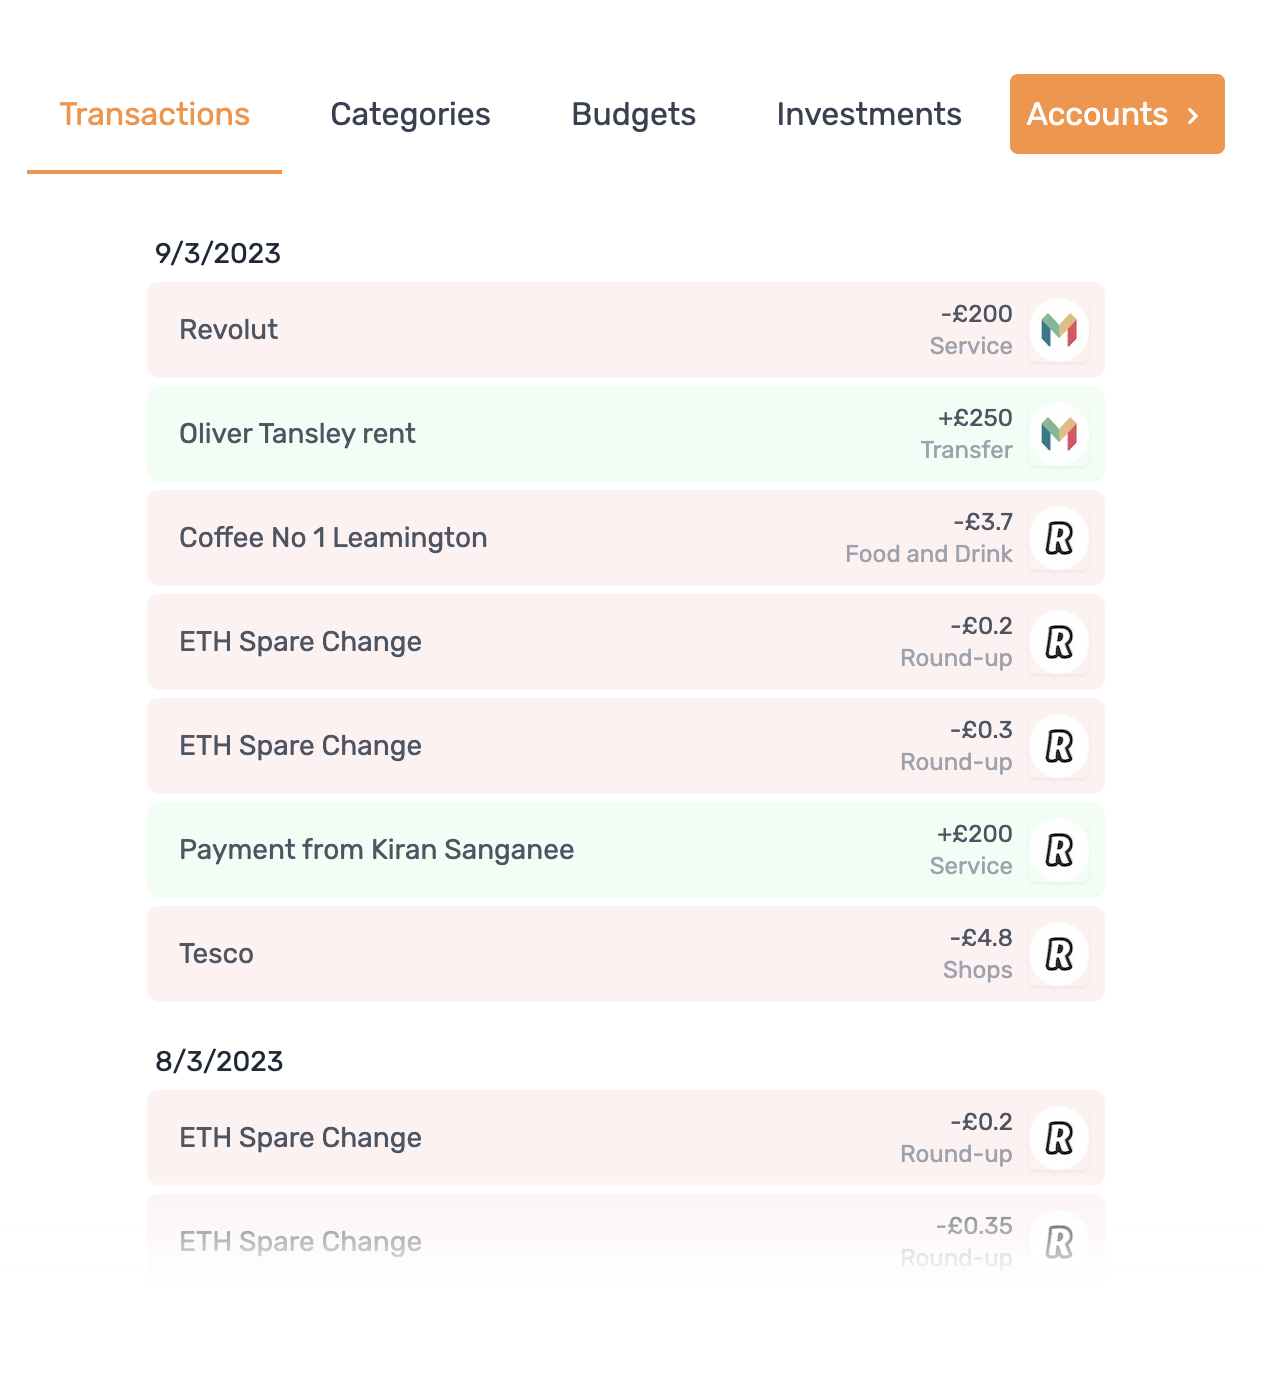
\includegraphics[width=\textwidth]{images/Transactions_development.png}
	\caption{Transactions strategy in development mode}
	\label{fig:TransactionsStrategy}
\end{figure}

The above figure (\ref{fig:TransactionsStrategy}) is an example of what the transactions look like in development mode with two separate bank accounts enabled. Each transaction has its own bar and displays information that is relevant to help provide an overview. Income is coloured light green, expenditure is coloured light red; yet when whichever transaction is hovered over is coloured slightly darker for UI feedback. Often enough transactions are shown that scrolling is required, however there was not a consistent way to style the scroll bar as it is dependent on the browser. To account for this, instead the scroll bar was removed entirely, but the bottom-most viewable transactions has an opacity gradient to indicate there are more transactions below.

\subsection{Categories}
This sprint followed on easily from the transaction sprint as much of the backend functionality could be reused. For this strategy, only the expenditure needed to be analysed. One option was to modify the Next.js API route so that it separates the data into income and expenditure (by positive and negative value) automatically, however would have involved some slight changes to the transaction strategy. Instead, a similar but new Next.js API route was created to get the expenditure data only. This also acted as an optimisation as the categories strategy only needed the previous thirty days of transactions so speed up the data processing by creating a different API route.

\begin{figure}[H]
	\centering
	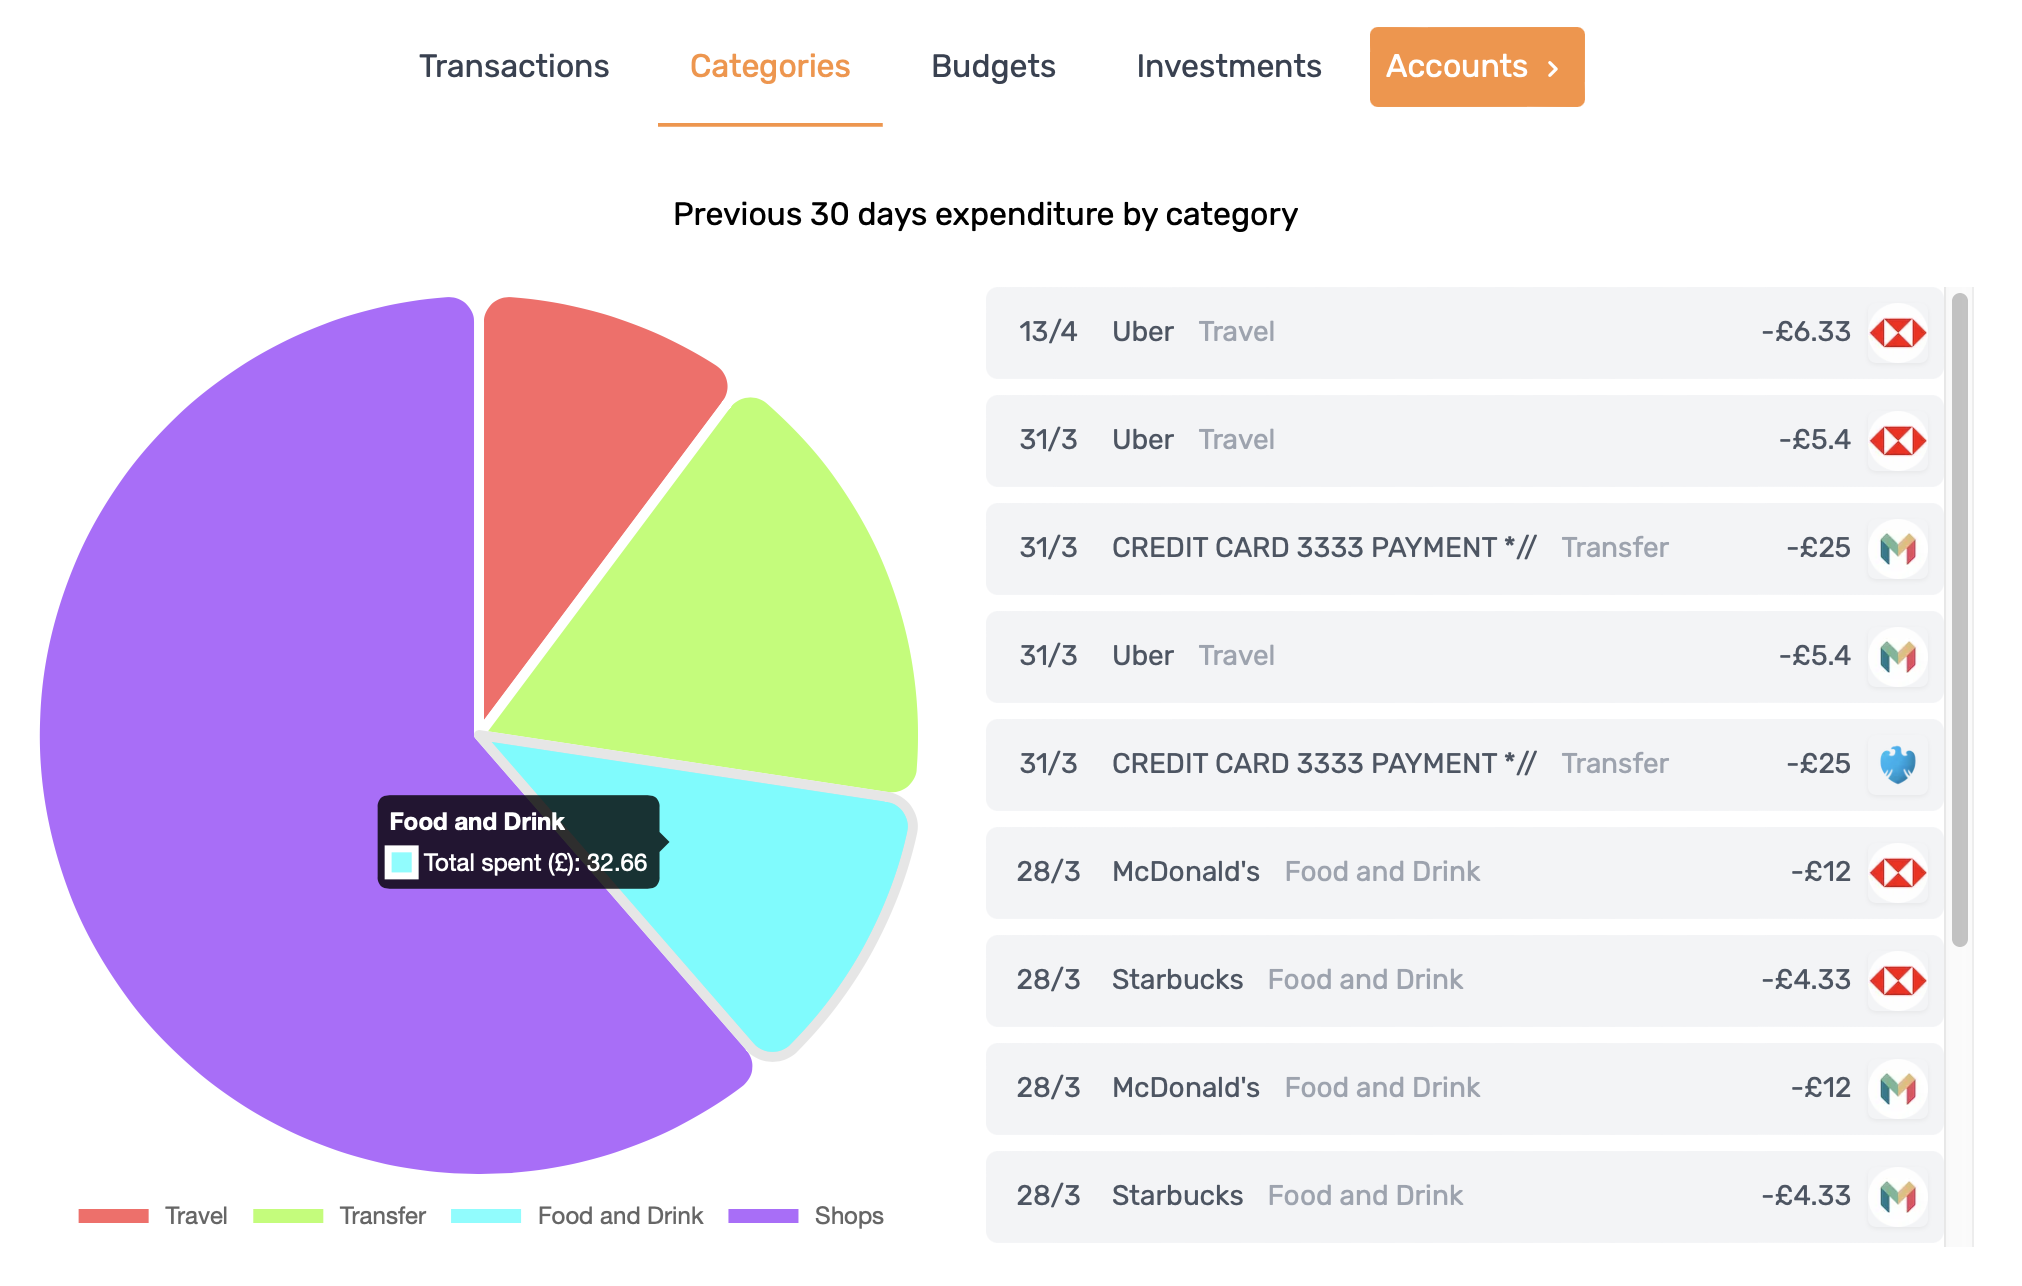
\includegraphics[width=\textwidth]{images/Categories_sandbox.png}
	\caption{Categories strategy in sandbox mode}
	\label{fig:CategoriesStrategySandbox}
\end{figure}

The above figure (\ref{fig:CategoriesStrategySandbox}) is an example of what the categories look like in sandbox mode with four accounts enabled. On the left is a dynamic pie chart that shows the relative amounts each category makes up for the past thirty days. The colours are intelligently chosen; in the above example, there are a total of four categories, so four different colours are chosen which are most distinguishable from each other. In the figure, the user is hovering over the light blue section which is 'Food and Drink', so the total for this section is displayed. On the right is the list of all expenditure for the past thirty days but these are not grouped at all, and there is an emphasis on the category; unlike in the transactions strategy.

The below figure (\ref{fig:CategoriesStrategyDevelopment}) is an example of what the categories look like in development mode with two accounts enabled. In this case the pie chart is more realistic as is made up of real data. In addition, a filter has been applied to the categories to only show expenses in the 'Food and Drink' category. To apply this filter, the user has simply clicked on the 'Food and Drink' category in the pie chart; to remove the filter, they can just click the red trash icon above the expenses.

\begin{figure}[H]
	\centering
	\makebox[\textwidth][c]{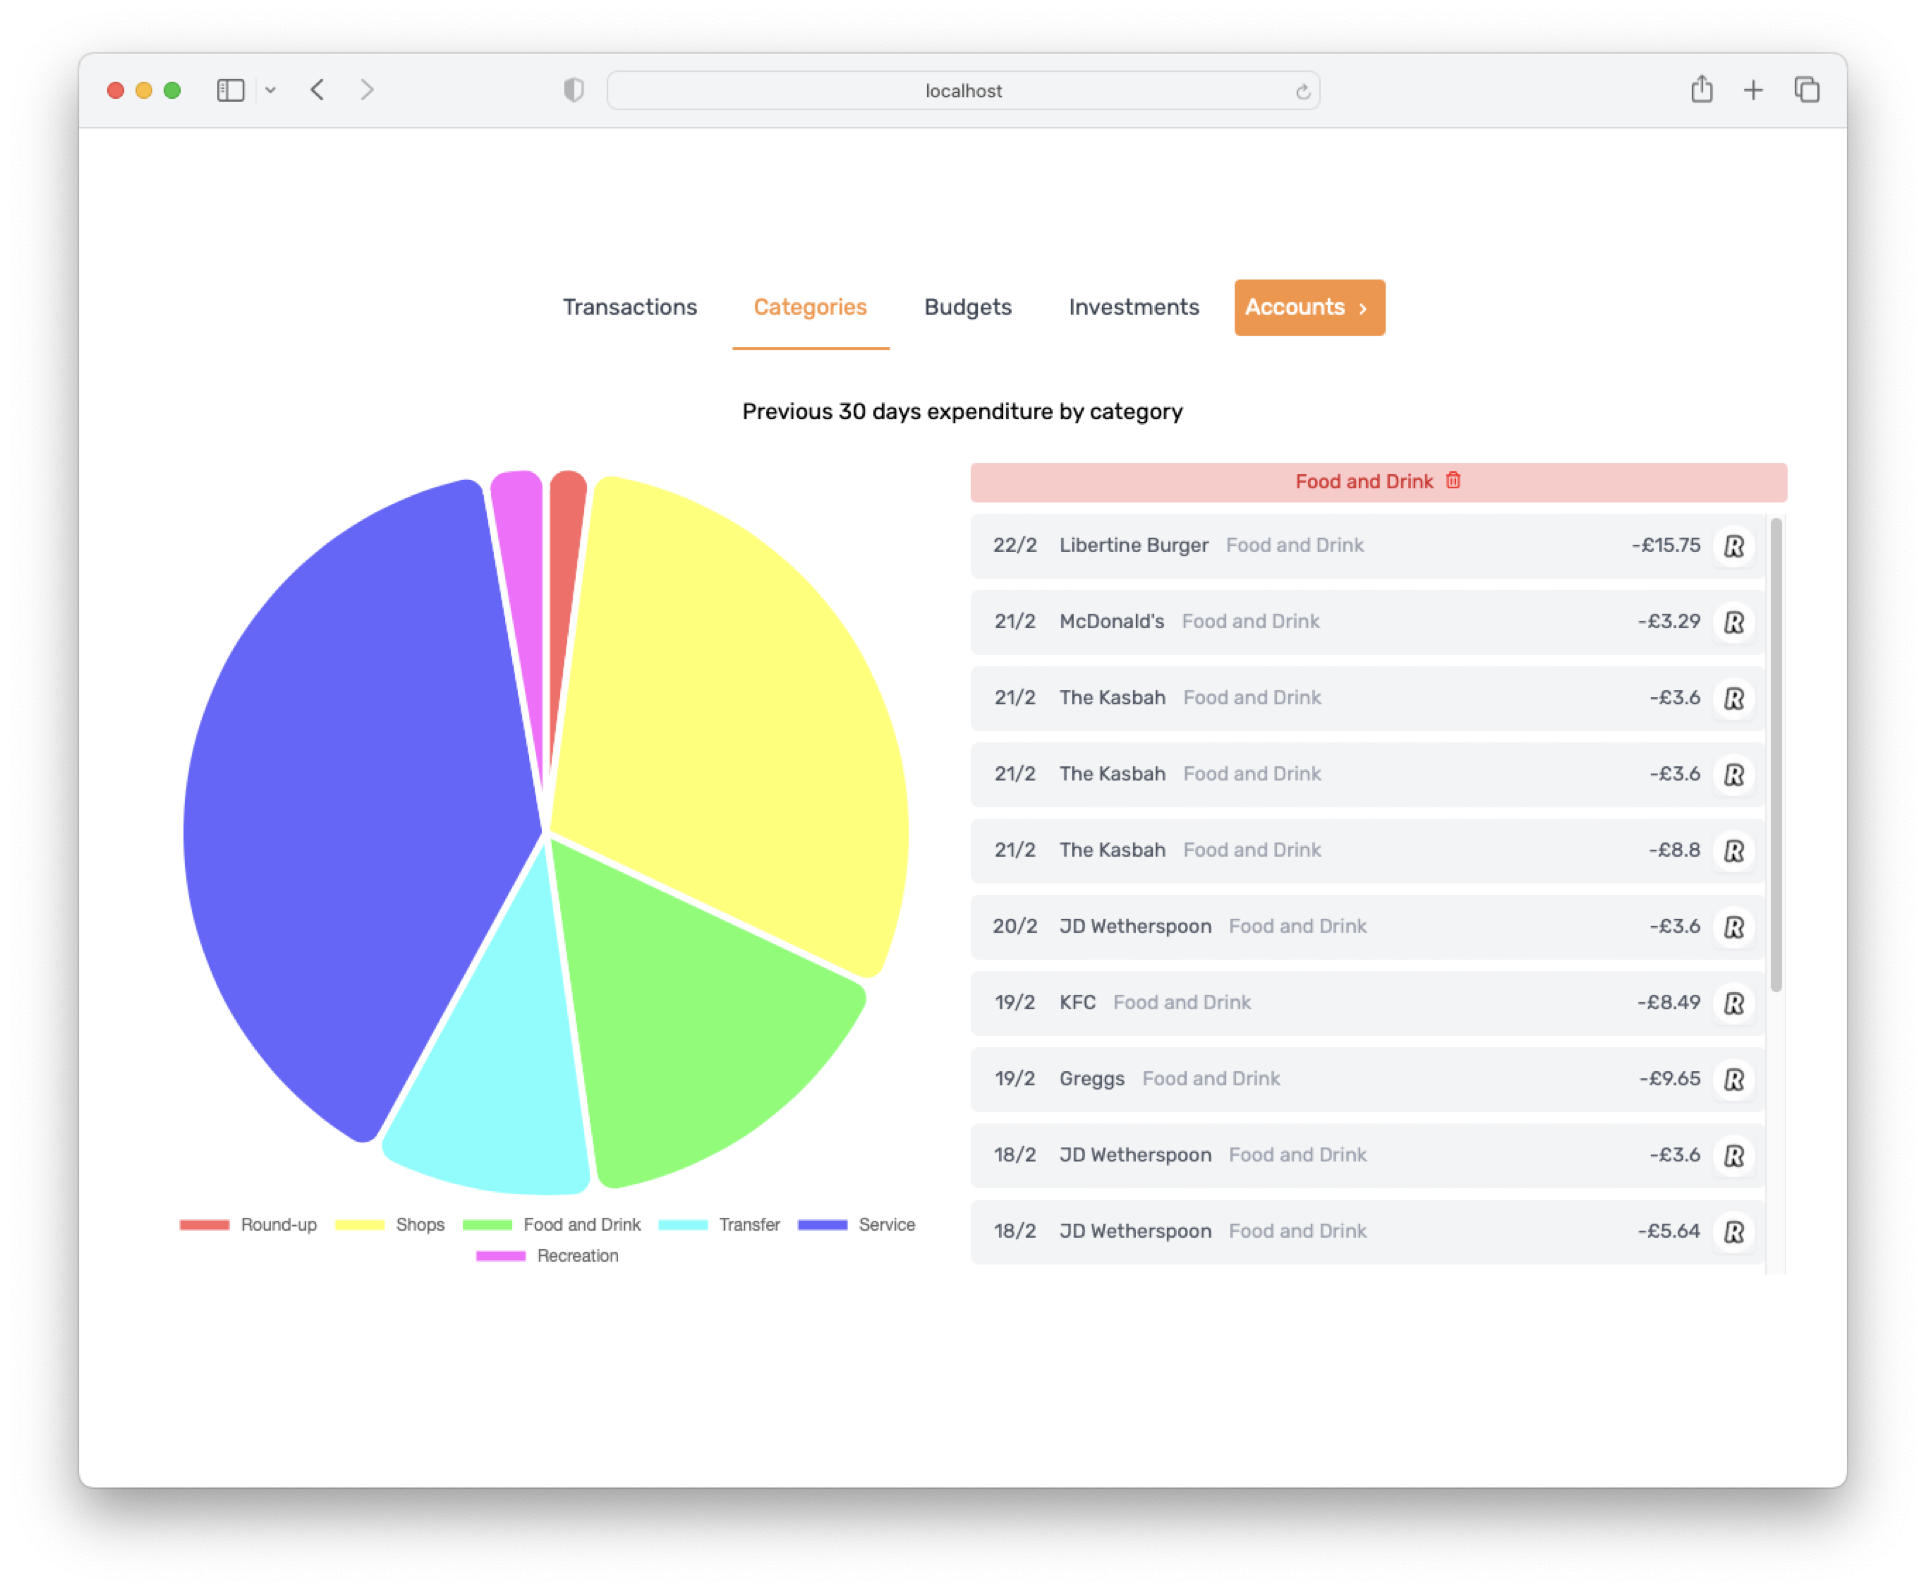
\includegraphics[width=1.1\textwidth]{images/Categories_development.png}}
	\caption{Categories strategy in development mode with a filter}
	\label{fig:CategoriesStrategyDevelopment}
\end{figure}

\subsection{Budgets}
In the original sprint for the budgeting strategy, there was no budget prediction. Instead the sprint resulted in a graphical view of the previous expenditure by displaying the amount spent each day, with a total amount on the side. The user could also enter an amount to budget for the month, and on the line chart, this budget would be displayed. The research portion of this sprint did identify that budget prediction was a useful feature, but it was not considered initially as would involve more time than the single sprint. After the end of the investment sprint, the budget strategy seemed lacking so a new phase was proposed to incorporate budget prediction.

\subsubsection{Time Series Forcasting}
As mentioned in design section (\ref{ch:design}), the best option for budget prediction was to use a neural network. The decision that was most key in turning the problem of budget prediction, into a more well defined problem was to turn the expenditure data into cumulative amounts spent. This altered the data into a time series and meant that there was much more research and literature available on how to tackle this kind of problem. The cumulative amounts would also reset every month to match the budgeting period, but also made no difference to the model as the model would learn this.

The book Forecasting: Principles and Practise (3rd edition) \cite{ForcastingPrinciplesPractise} was a particularly useful resource for this section. Not only did it talk about the effects of seasonal time series - in this case is the cumulative resets, but also about how to apply linear regression techniques (which helped in the deciding to use a neural network) and using a neural network to make predictions.

\subsubsection{Long Short-Term Memory}
The term that often repeatedly cropped up during the research was LSTM, meaning Long short-term memory. They are "a type of recurrent neural network capable of learning order dependence sequence prediction problems" \cite{LSTMGentleIntro}. The cumulative data could be seen as a order dependent sequence, and the problem is just predicted the next value to appear in the sequence. 

What makes LSTM's different from ordinary recurrent neural networks is that the individual units have single value memory cells that can be controlled by three gates. The first gate is an input gate which determines if the current value in the cell should be summed into memory. The second gate is the output gate which determines if the memory is added to the input as output. The final gate is the forget gate which determines if the memory should be cleared. The weights which dictate if these gates are open or closed are learnt along with the other weights in the network.

\subsubsection{Training}
To train the LSTM model, the input training data consisting of the past three years of transactions first needed to be modified. The data was turned into the cumulative data and resetting at 0, but in addition it was split in such a way to maximise the amount that could be learnt. This was done by taking the first value up to the thirtieth value as one training example, and the thirty-first value being the predicted output. Then by taking the second value up to the thirty-first value as the next training example, and the thirty-second value being the predicted output. This was done for up to the end of the data resulting in 1064 training examples. Techniques such as test-train split and validations sets were also used.


\subsubsection{Architecture}
Throughout the research and testing phase, LSTM models were found to be the most accurate relative to other neural network architectures as well as other machine learning models like linear regression. This also complimented the fact that there is support for LSTM models in the Keras library. The structure of the network that was found to be the sufficiently simple that it could be trainined in a realistic amount of time, but also sufficiently complex to be able to learn the data was a single LSTM layer with 64 units, followed by a dense layer with 1 unit as output. To make the predictions realistic, but not too overfit on the training data, 30 epochs were used to train the model. Finally, a window size of 30 was used, meaning the model has 30 inputs, as to match the modified training data and budgeting period.

\subsubsection{Results}
\begin{figure}[H]
	\centering
	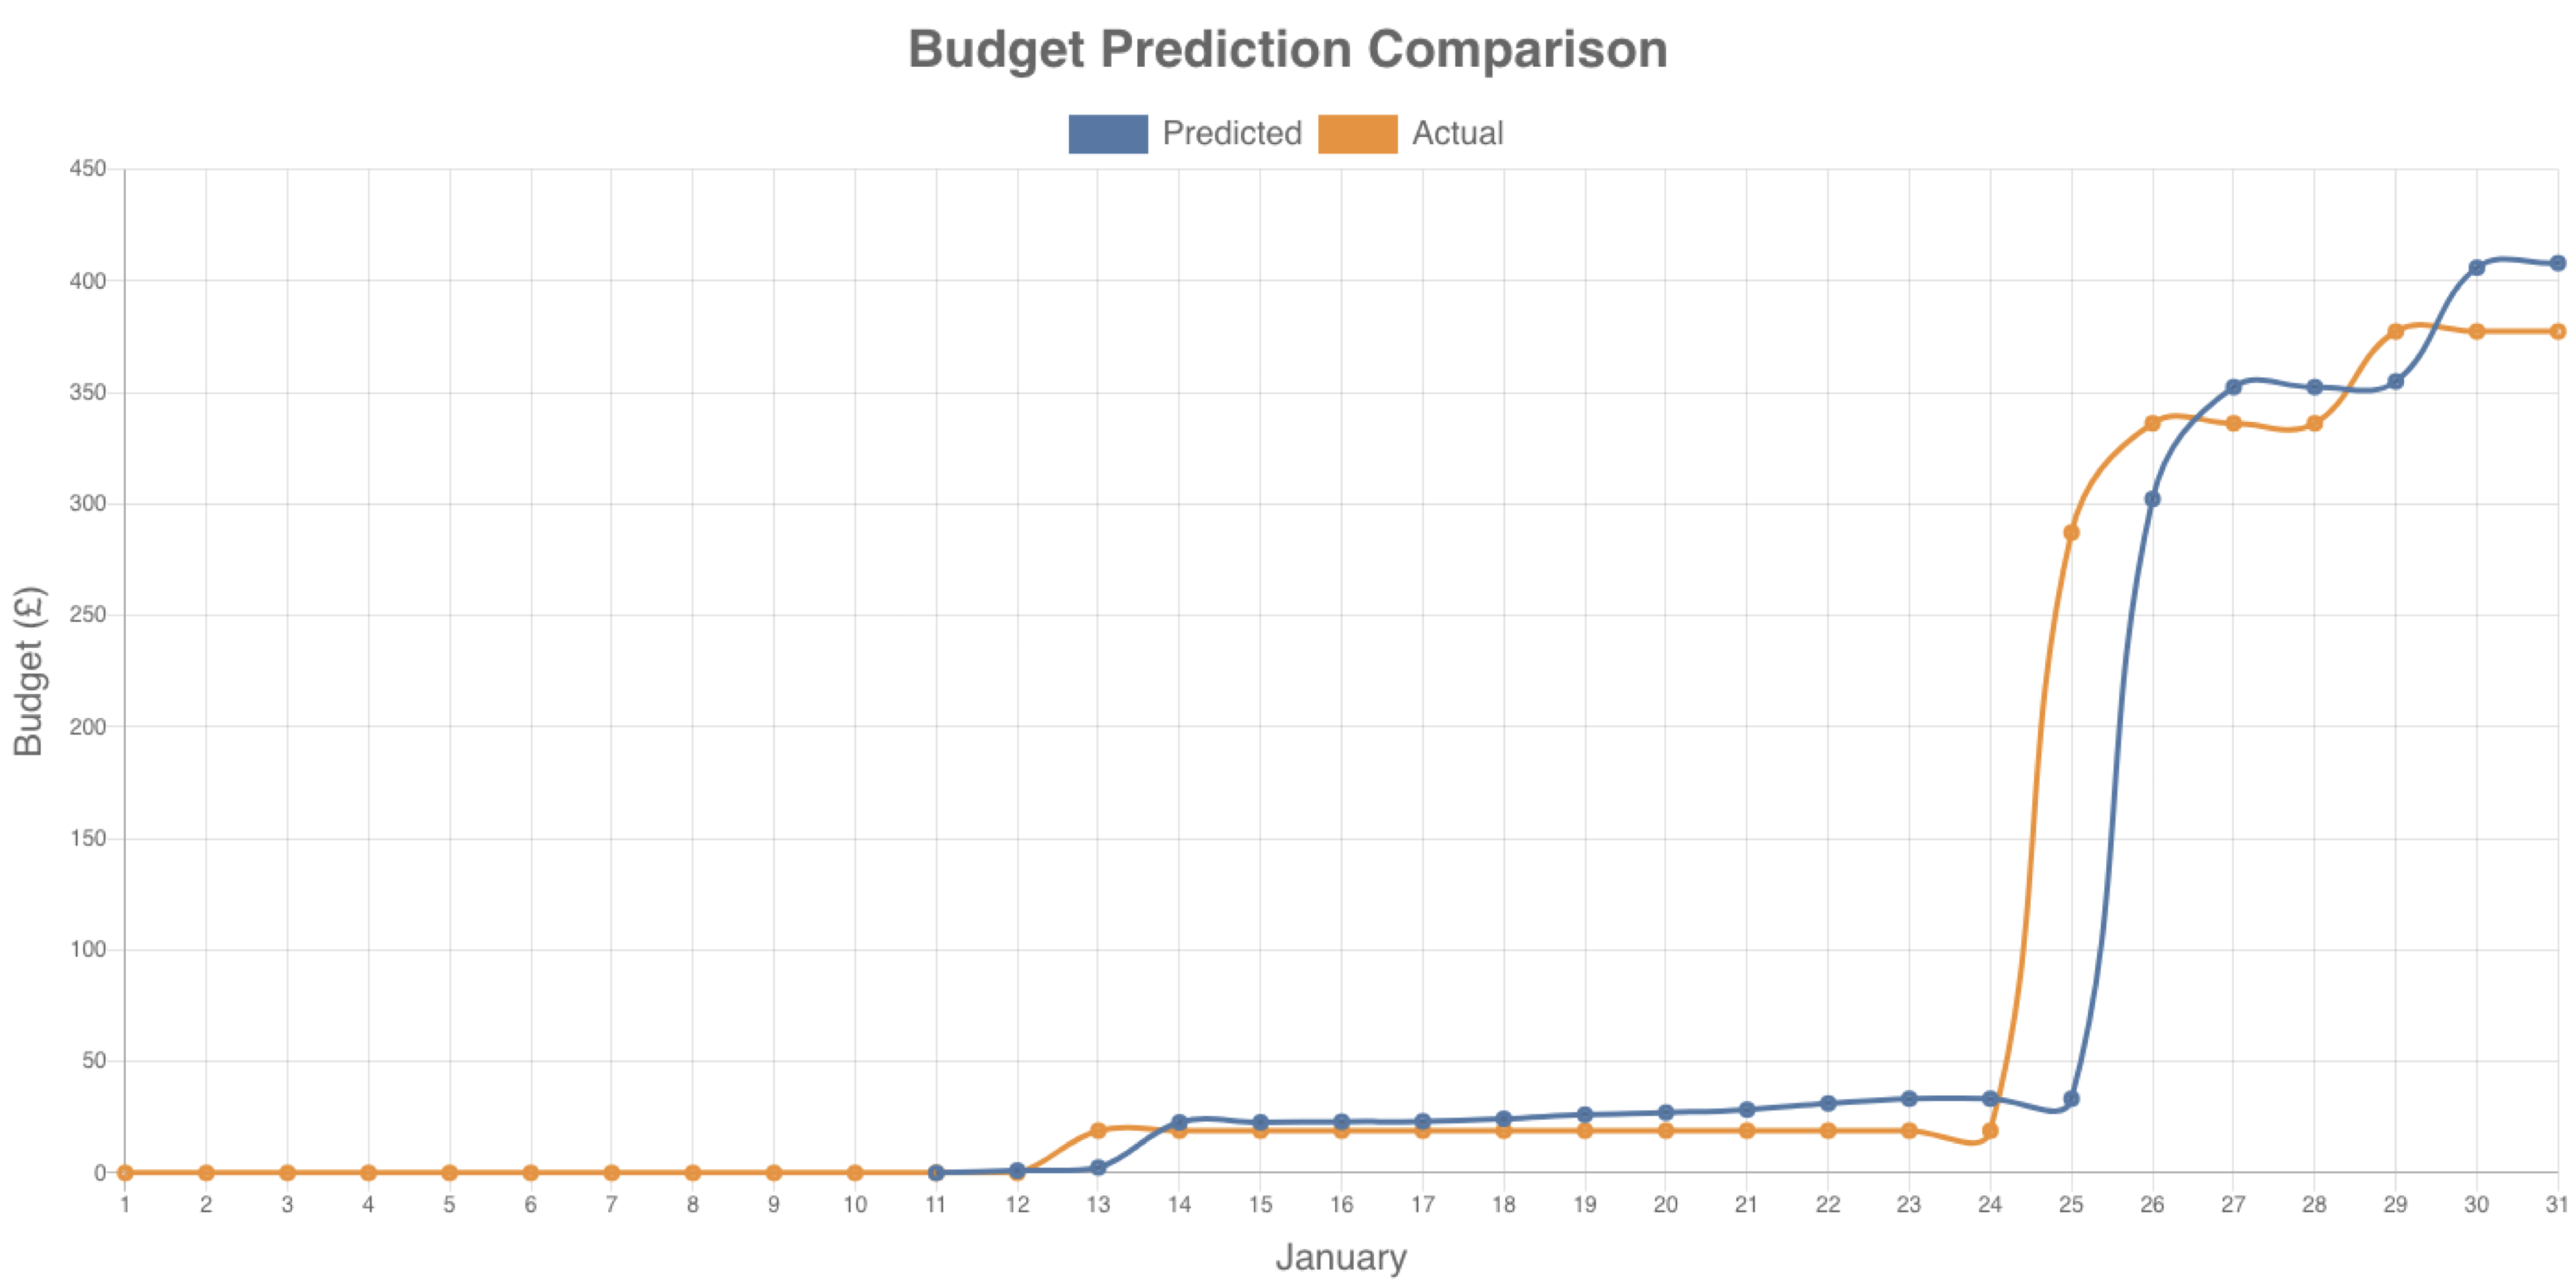
\includegraphics[width=\textwidth]{images/Budger_prediction_comparison.png}
	\caption{Budget prediction results}
	\label{fig:BudgetPredictionResults}
\end{figure}

The above figure (\ref{fig:BudgetPredictionResults}) displays the difference between the predicted expenditure vs the actual expenditure. In this instance, the data used for this graph is the fake data generated by Plaid, so isn't even related to the data that the model was trained on. The model was able to predict the expenditure very accurately, and also followed the pattern effectively. There is a slight offset in the two lines, but this eventually was found out to be due to the way Plaid generate their transactions. They assume that each month has thirty days in it, but the graph is for the month of January which has thirty-one days, explaining the offset.

\subsubsection{Budget Strategy}
Using this accurate budget prediction model, it is incorporated into the budget strategy by making predictions for the rest of the month. Suppose the user is accessing the tool on the 15th day of the month. For the past fifteen days, the tool will have access to their actual transactions and can plot the cumulative expenditure. For the remaining days in the month, a prediction is made and plotted.

The prediction is made by taking the past 30 days expenditure and predicting the amount on the 16th day of that month. Then using this predicted value and the true past 29 days of expenditure, an amount is predicted for the 17th, and so on. All of these values are then displayed to the user in the graph which they can compare to their budgeted amount.

\begin{figure}[H]
	\centering
	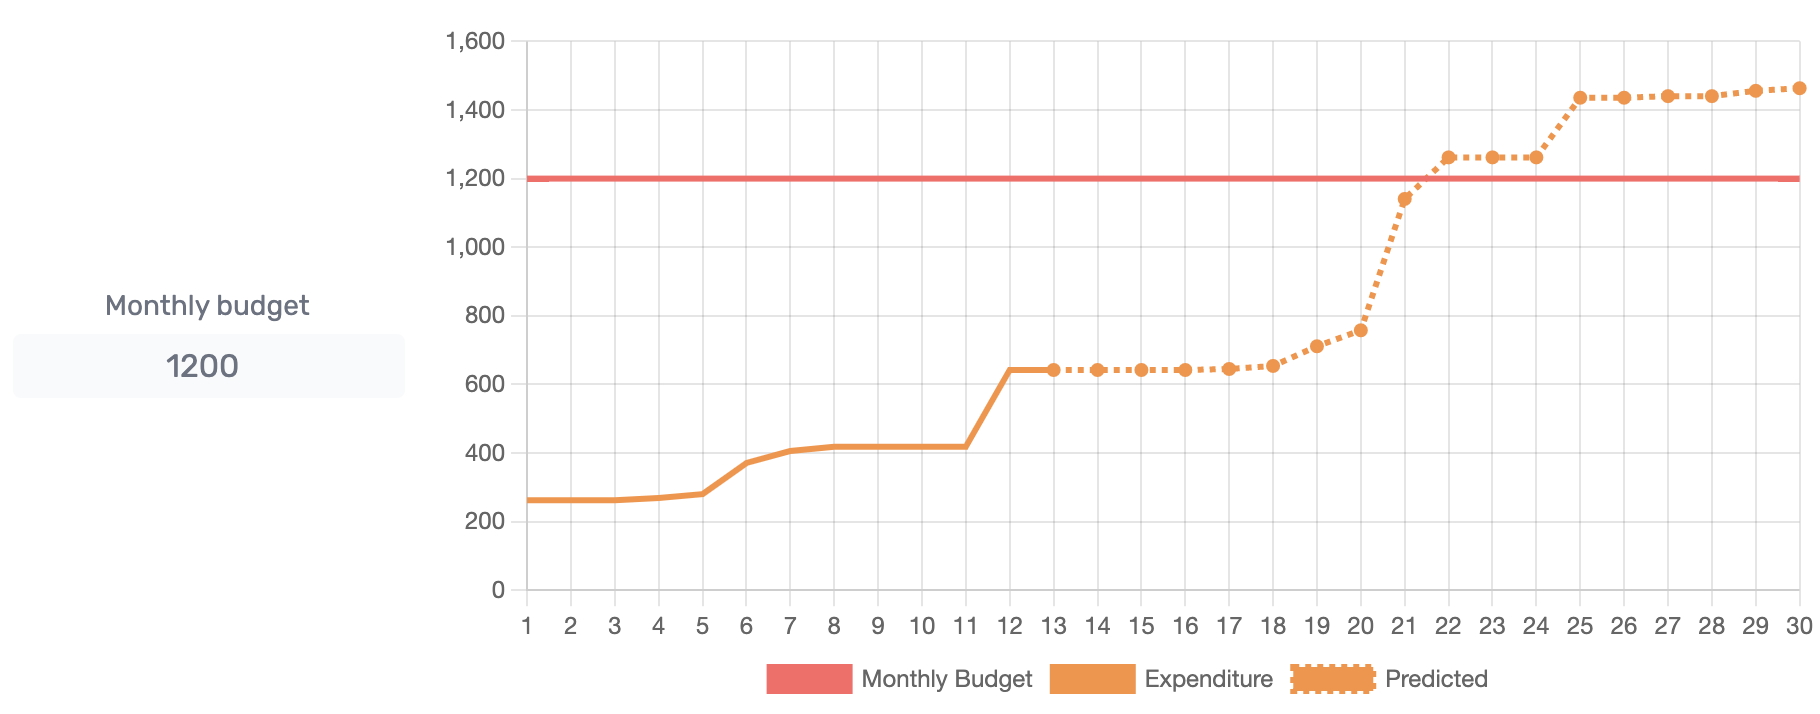
\includegraphics[width=\textwidth]{images/Budget_strategy.png}
	\caption{Budget strategy in development mode}
	\label{fig:BudgetStrategy}
\end{figure}

The figure above (\ref{fig:BudgetStrategy}) shows the budget strategy in development mode with the budget prediction incorporated. The date of access is the 13th April, so there is actual expenditure up to this date. The remaining days contain the predicted expenditure. The set monthly budget is \textsterling 1200, but according to the graph, it is predicted that they wil exceed their budget so should make adjustments accordingly.

\subsection{Investments}
The final sprint before the last phase was dedicated to implementing the investments strategy. As outlined in the design phase (\ref{ch:design}), the aim for this section was to give an overview of the user's portfolio. Unlike the other strategies, this one didn't use Plaid, so a needed a lot more custom functionality.

The user is expected to add their investment initially, however the tool should automatically update following this. This meant storing the investment in the database. To accommodate for this, a new Next.js endpoint was required which would take the relevant information about the asset, such as ticker and the price it was bought for, and stores is in the database. Like the access tokens, this entry is linked to the user's account is is only accessible by the creator of the entry. Similarly, another endpoint was required to retrieve all the investments for a user and one to delete an investment.

When a user accesses the investment strategy, the UI should display all of their added investments. This a request is made to the new endpoint to get the investments. For each investment, once the stored data is retrieved, it will then access a live API to get the actual current price fo the asset. This used to calculate the profit and percentage change. For an investment that has made profit, it is shown in a light-green like income in the transactions strategy. An investment that has made a loss is shown in a light-red like expenses also in the transactions strategy. Each investment also has a delete button which calls the delete endpoint and updates the UI accordingly.

When accessing the Financial Modelling Prep service, the information retrieved from the database can still be displayed. This means that initially a loading icon is displayed for the data that takes longer to access. The figure below (\ref{fig:InvestmentsLoading}) shows the table with demonstration information retrieved from the database, but still loading the actual price. The figure below this (\ref{fig:InvestmentsLoaded}) shows the table once the investments have been loaded and profits calculated. Each investment is treated independently, this means that they can load independently and so if one investment takes longer to load, the others will still be displayed as soon as they are ready.

\begin{figure}[H]
	\centering
	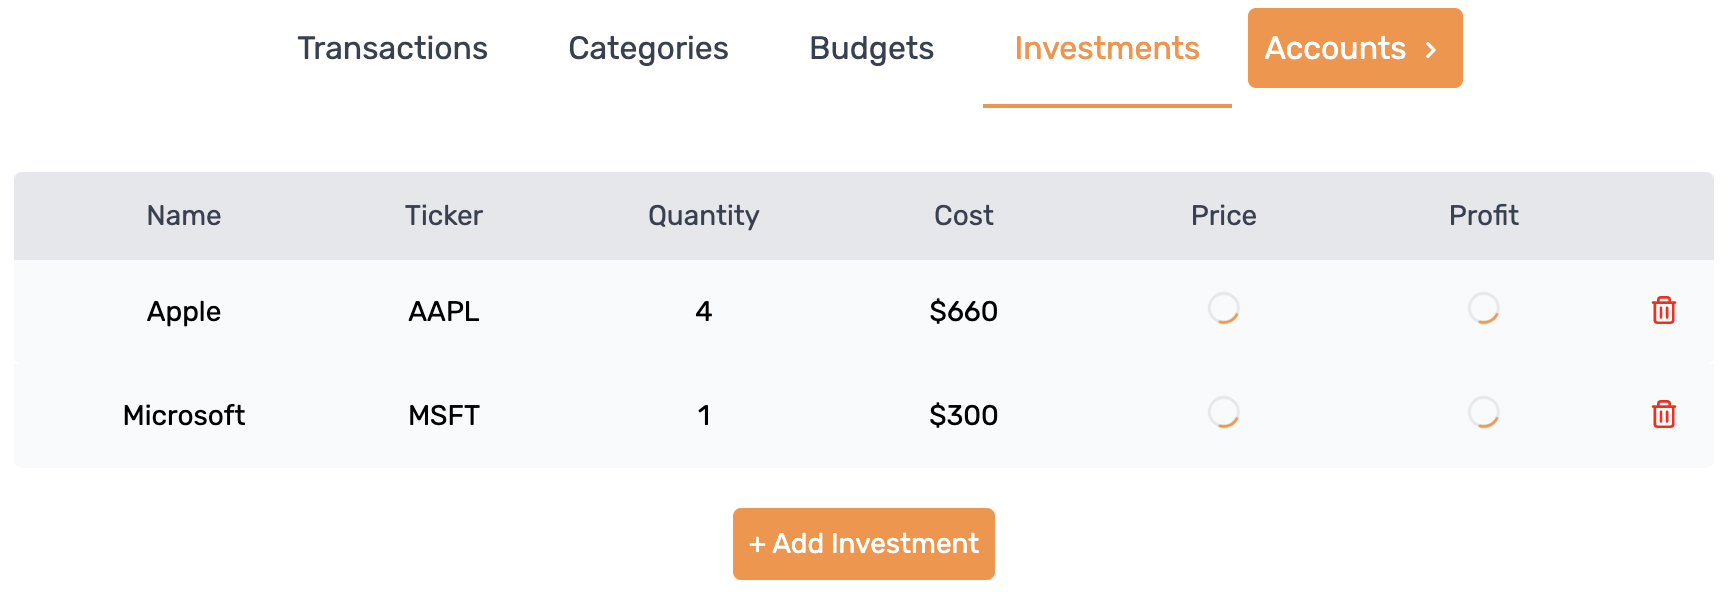
\includegraphics[width=\textwidth]{images/Investments_loading.png}
	\caption{Investments loading}
	\label{fig:InvestmentsLoading}
\end{figure}

\begin{figure}[H]
	\centering
	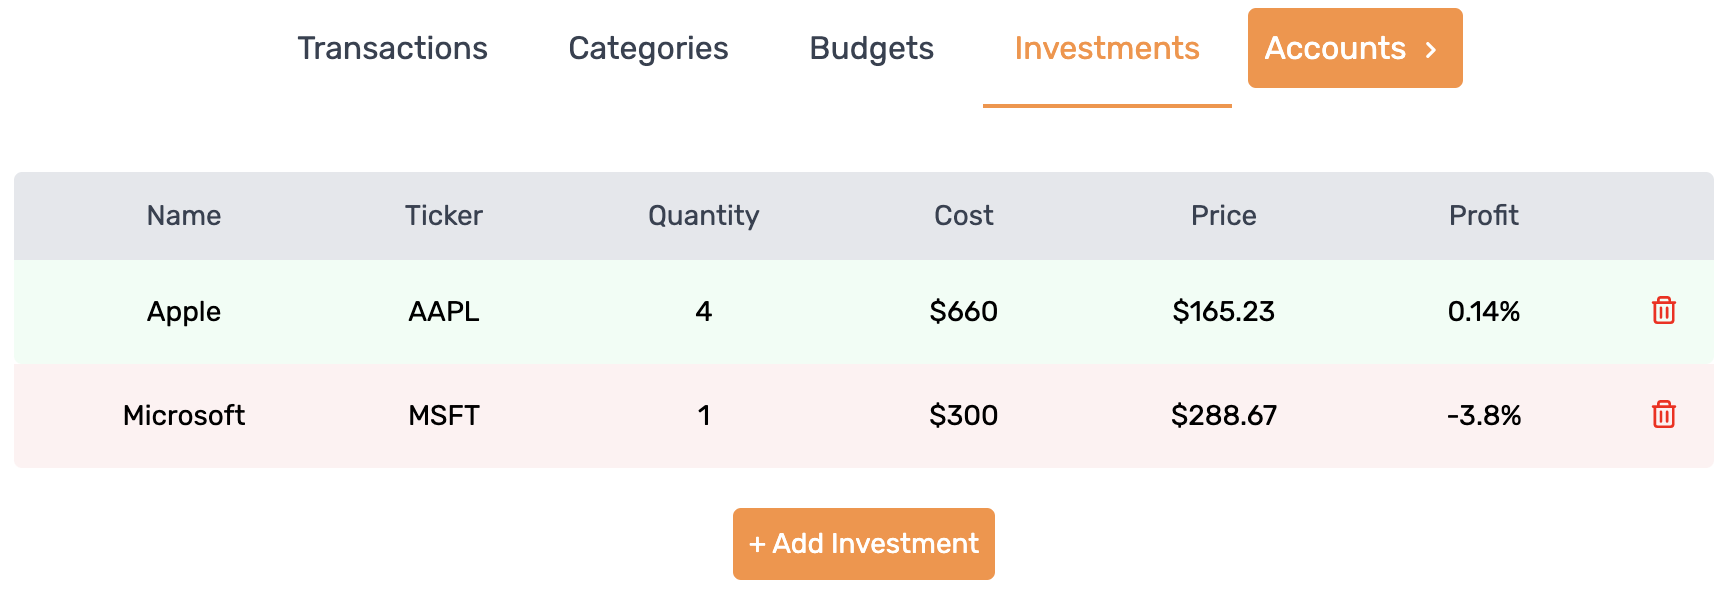
\includegraphics[width=\textwidth]{images/Investments_loaded.png}
	\caption{Investments loaded}
	\label{fig:InvestmentsLoaded}
\end{figure}

The table of investments has a max height, this means that if the user has a lot of investments, they do not extend the page downwards to display them all. Instead the table is made scrollable. This is to allow a portion of the UI, below the table, to be for how the user adds an investment. The ticker is a dropdown and allows the user to select a supported ticker (effectively an investment identifier). The user can enter the quantity and the amount they paid for the investment. Once a ticker is selected, when entering, the price is automatically filled in with the current price as an aid. These inputs all have client-side validation to ensure the user enters acceptable data. If it does not pass the validation, the box will turn red as a visual indicator of what is wrong, so can be corrected. Once the user has entered this information, they can click the add investment button which adds it to the table above as well as the database.

\begin{figure}[H]
	\centering
	\makebox[\textwidth][c]{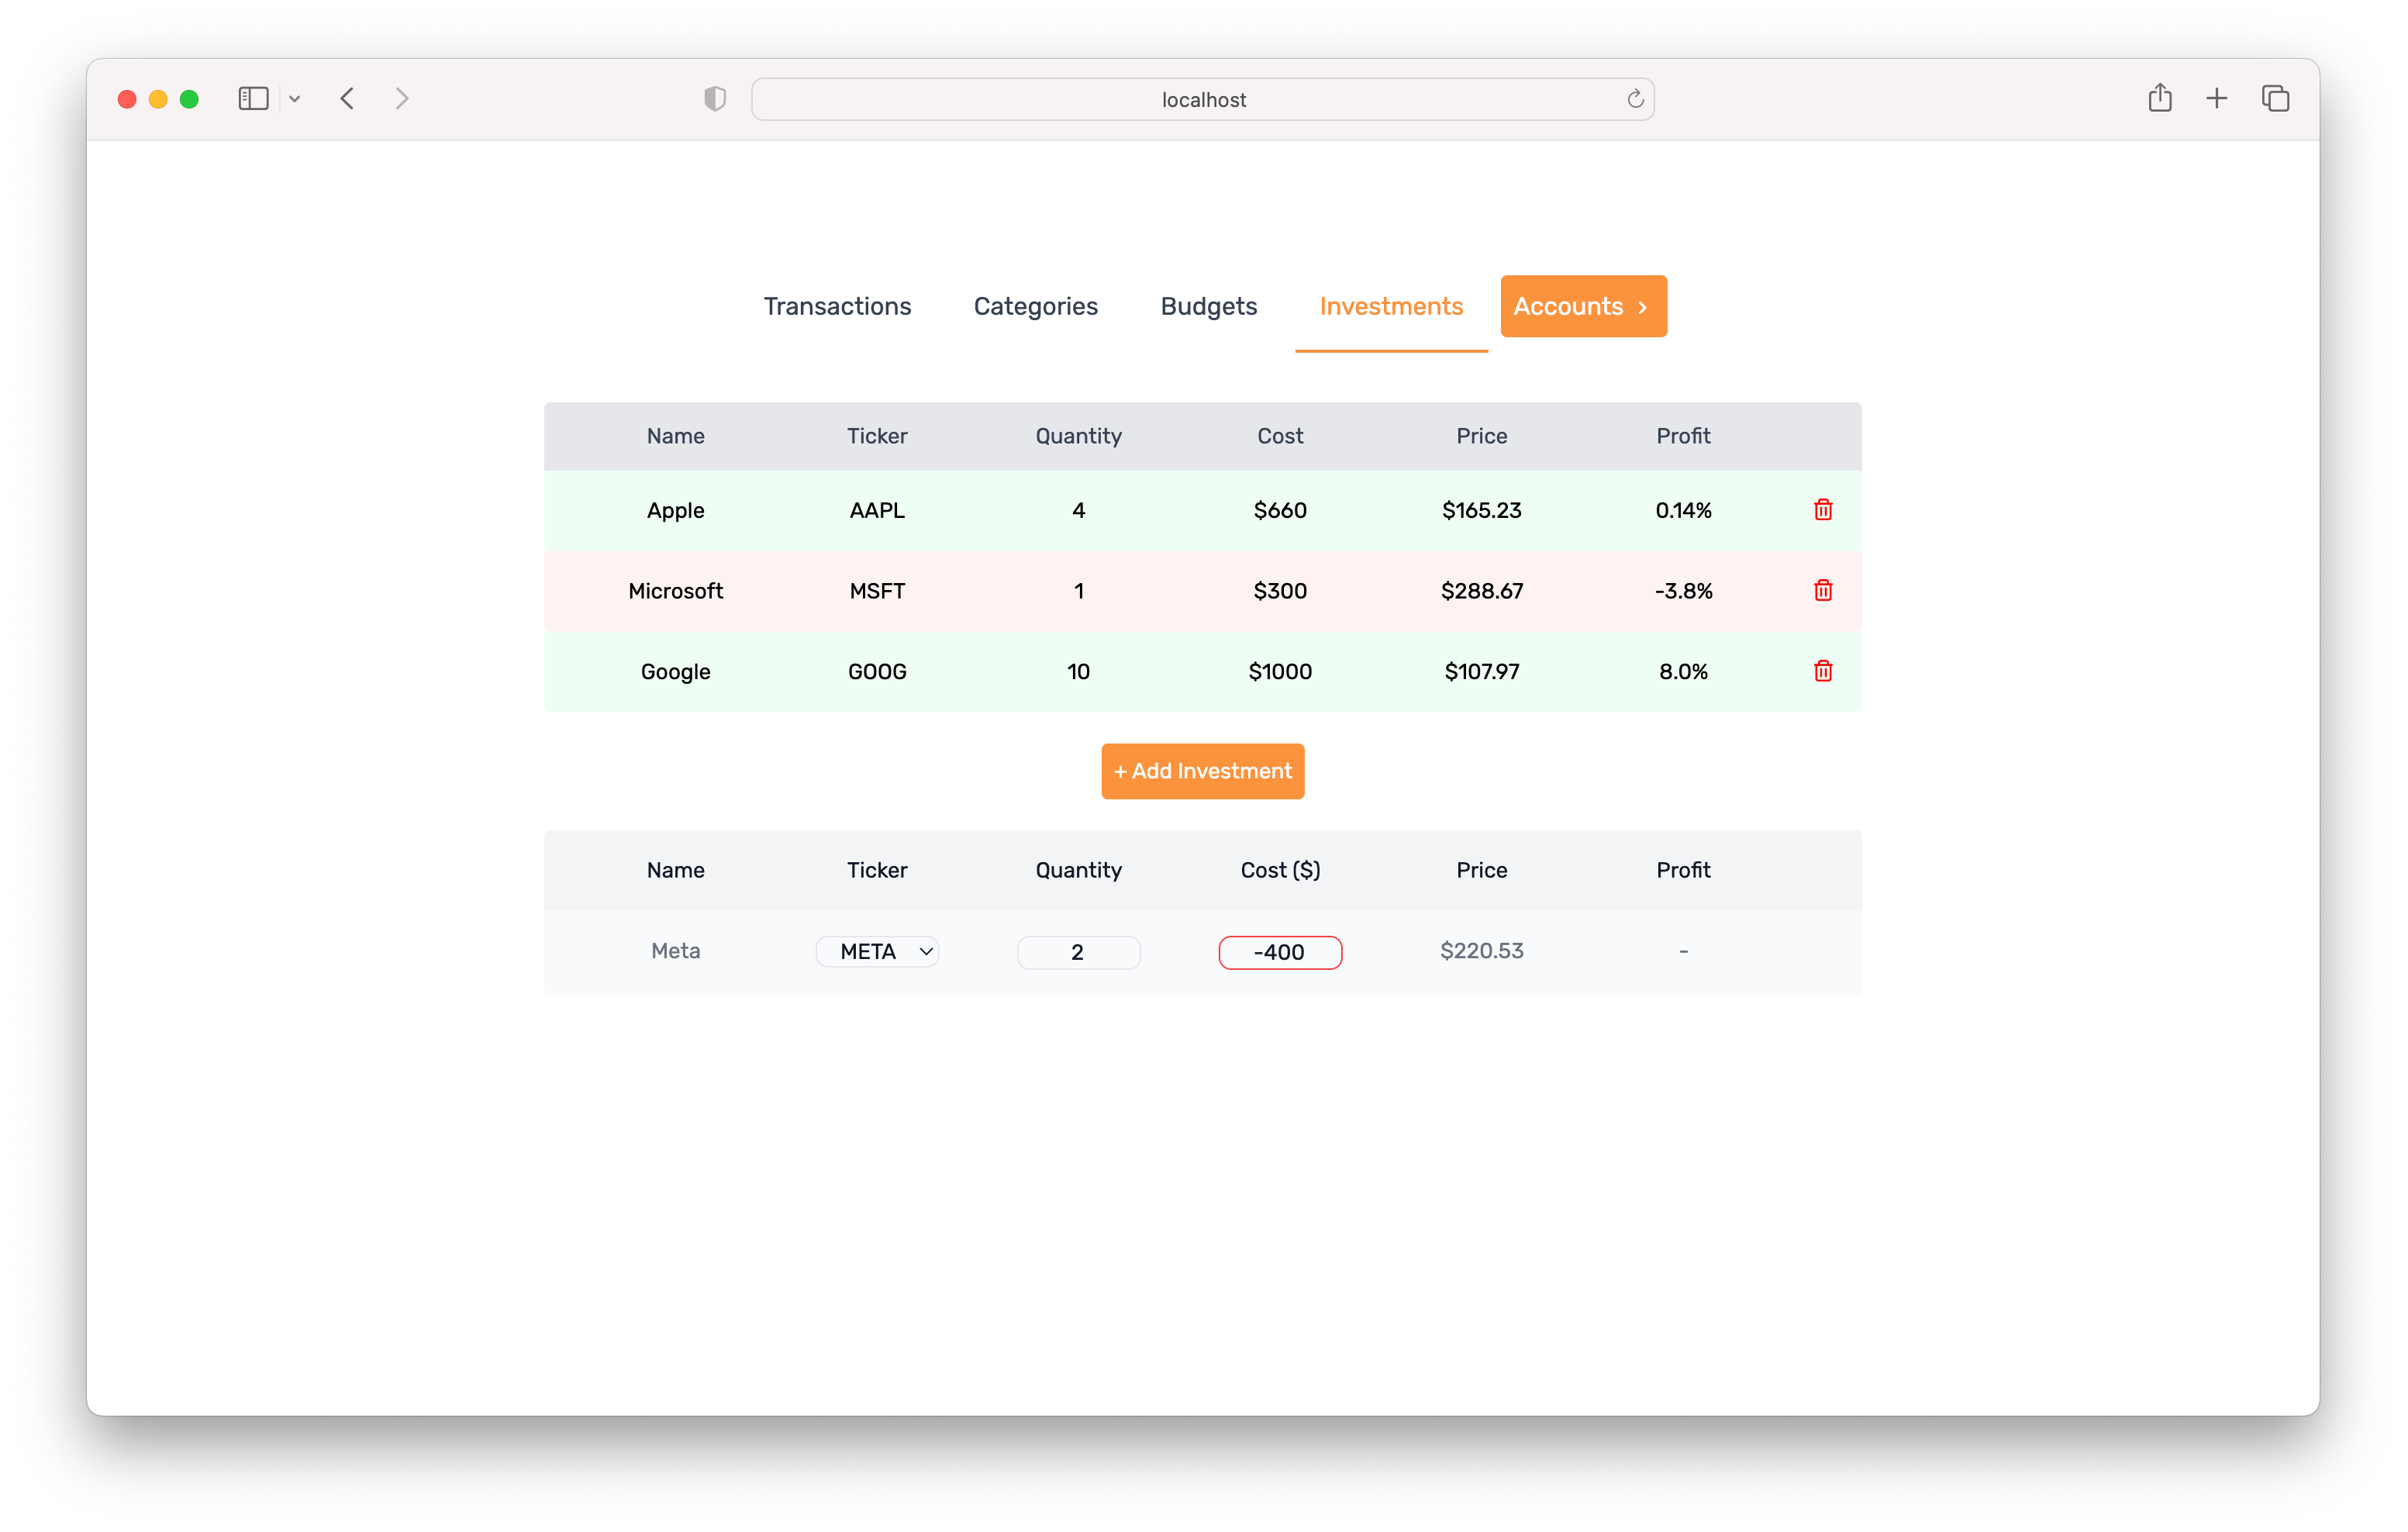
\includegraphics[width=1.1\textwidth]{images/Investments_error.png}}
	\caption{Adding an investment}
	\label{fig:InvestmentsError}
\end{figure}

The figure above (\ref{fig:InvestmentsError}) shows the user attempting to add a Meta investment. Everything is valid, except for the cost which has been mis-typed with a negative sign. This is picked up by the validation and the box turns red. The user can then correct this, then click the button and the investment will be added to the table.

\section{Endpoints}
\begin{figure}
	\centering
	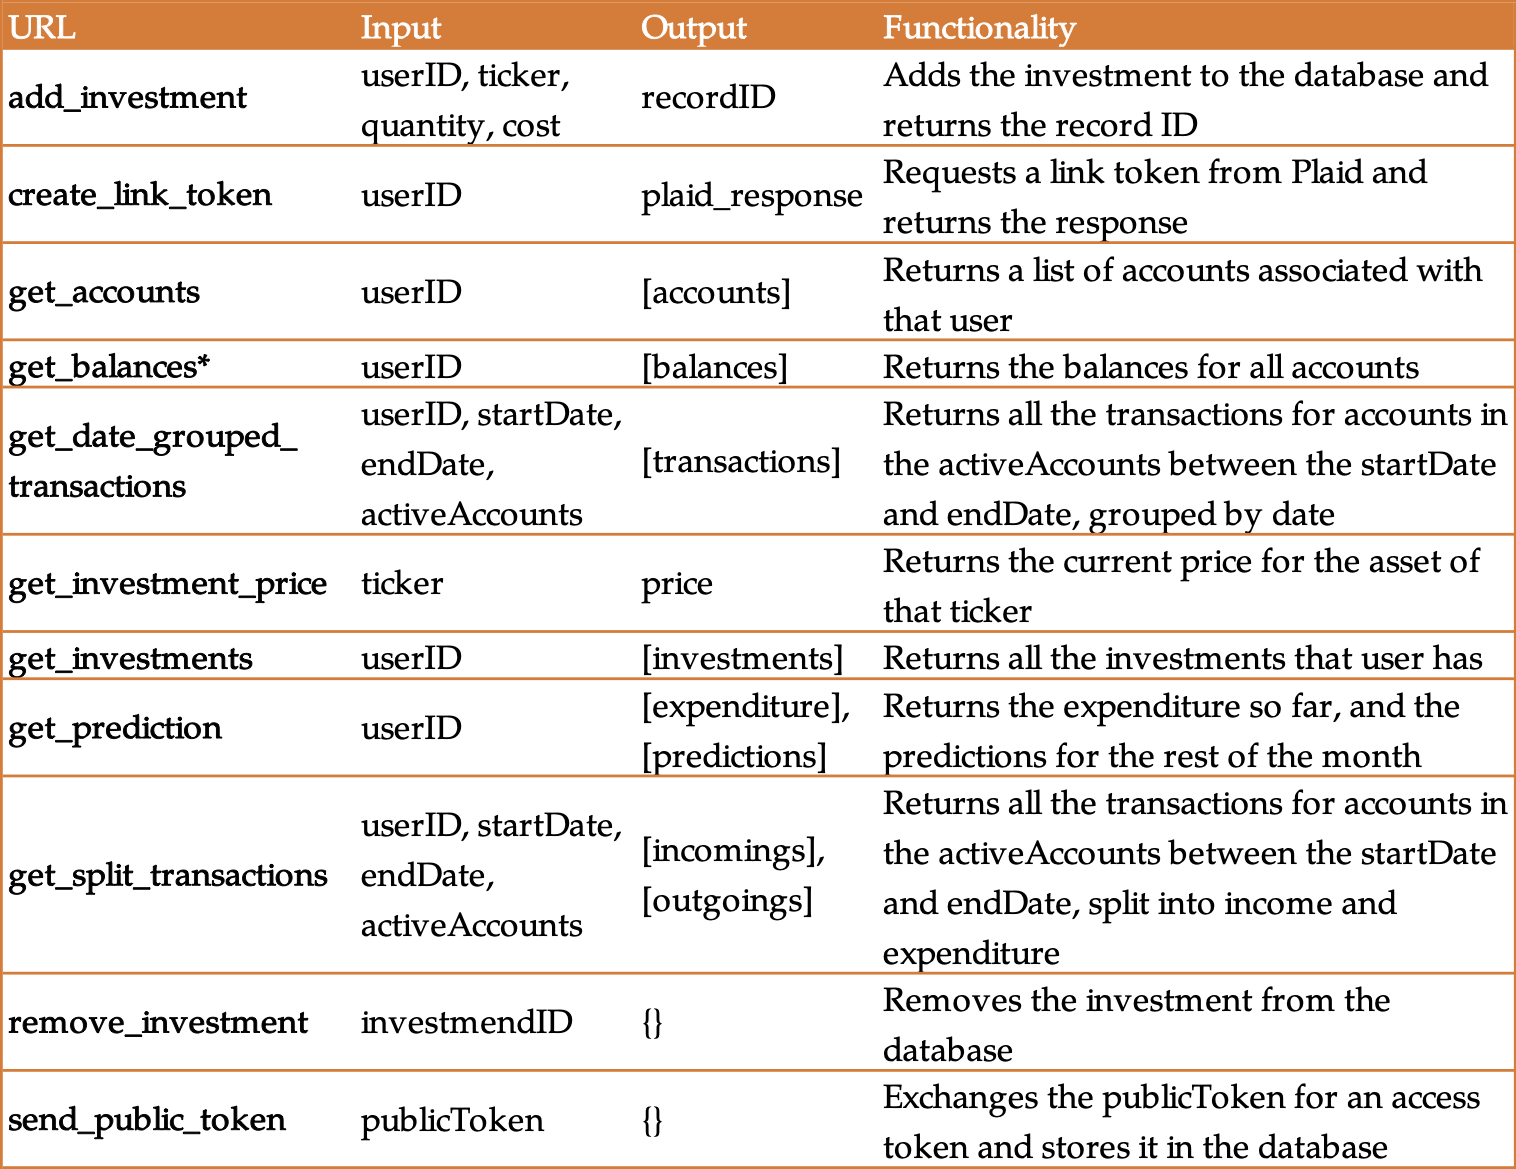
\includegraphics[width=\textwidth]{images/Endpoints.png}
	\caption{Endpoints}
	\label{fig:Endpoints}
\end{figure}
